\let\lesson\undefined
\newcommand{\lesson}{\phantomlesson{Bài 14.}}
\setcounter{section}{2}
\section{Trắc nghiệm nhiều phương án lựa chọn}
\setcounter{ex}{0}
\Opensolutionfile{ans}[ans/VN10-Y24-PH-SYL-023P-TN]
% ===================================================================
\begin{ex}\mkstar{1}
	Lực tác dụng vào vật làm cho vật quay quanh một trục có giá
	\choice
	{song song với trục quay}
	{cắt trục quay}
	{nằm trong mặt phẳng song song với trục quay}
	{\True nằm trong mặt phẳng vuông góc với trục quay và không cắt trục quay}
	\loigiai{Lực tác dụng vào vật làm cho vật quay quanh một trục có giá nằm trong mặt phẳng vuông góc với trục quay và không cắt trục quay.}
\end{ex}
% ===================================================================
\begin{ex}\mkstar{1}
	Cánh tay đòn của lực bằng
	\choice
	{khoảng cách từ trục quay đến điểm đặt của lực}
	{khoảng cách từ trục quay đến trọng tâm của vật}
	{\True khoảng cách từ trục quay đến giá của lực}
	{khoảng cách từ trọng tâm của vật đến giá của trục quay}
	\loigiai{}
\end{ex}

% ===================================================================
\begin{ex}\mkstar{1}
Một ngẫu lực gồm có hai lực $\vec F_1$ và $\vec F_2$, có $F_1 = F_2 = F$ và có cánh tay đòn $d$. Moment ngẫu lực này là	
	\choice
	{$(F_1-F_2)d$}
	{$2Fd$}
	{\True $Fd$}
	{Chưa xác định được}
	\loigiai{}
\end{ex}
% ===================================================================
\begin{ex}\mkstar{1}
Trường hợp nào sau đây \textbf{không} xuất hiện ngẫu lực tác dụng lên vật?	
	\choice
	{Dùng tua vít chữ T để vặn đinh ốc}
	{Điều chỉnh tay lái ô tô}
	{Dùng tay vặn núm công tắc điều khiển đài radio}
	{\True Đẩy thùng hàng lên một mặt phẳng nghiêng}
	\loigiai{}
\end{ex}
% ===================================================================
\begin{ex}\mkstar{1}
	Chọn nhận định đúng.\\
	Quy tắc moment lực 
	\choice
	{chỉ áp dụng được cho vật rắn có trục quay cố định}
	{chỉ áp dụng được cho vật rắn có trục quay không cố định}
	{\True áp dụng được kể cả vật rắn đang chuyển động tịnh tiến}
	{luôn làm cho vật quay theo chiều kim đồng hồ}
	\loigiai{}
\end{ex}
% ===================================================================
\begin{ex}\mkstar{2}
	Hai lực của ngẫu lực có độ lớn $F=\SI{20}{N}$, khoảng cách giữa hai giá của ngẫu lực là $d=\SI{30}{cm}$. Moment của ngẫu lực có độ lớn bằng
	\choice
	{$\SI{0.6}{\newton\cdot\meter}$}
	{$\SI{600}{\newton\cdot\meter}$}
	{\True $\SI{6}{\newton\cdot\meter}$}
	{$\SI{60}{\newton\cdot\meter}$}
	\loigiai{$$M=Fd = \SI{6}{\newton\cdot\meter}.$$}
\end{ex}
% ===================================================================
\begin{ex}\mkstar{2}
	Một vật rắn có trục quay cố định, khi tác dụng một lực có độ lớn $\SI{10}{\newton}$ lên vật và khoảng cách từ giá của lực đến trục quay là $\SI{20}{\centi\meter}$ thì moment của lực tác dụng lên vật có độ lớn là $M_1$, khi tác dụng một lực có độ lớn $\SI{15}{\newton}$ lên vật và khoảng cách từ giá của lực đến trục quay là $\SI{5}{\centi\meter}$ thì moment của lực tác dụng lên vật có độ lớn là $M_2$. Chọn hệ thức đúng.
	\choice
	{\True $3M_1=8M_2$}
	{$3M_2=8M_1$}
	{$3M_1=4M_2$}
	{$4M_1=3M_2$}
	\loigiai{}
\end{ex}

% ===================================================================
\begin{ex}\mkstar{2}
	Cho thanh OB đồng chất có khối lượng $\SI{5}{\kilogram}$ gắn vào tường nhờ bản lề tại O như hình vẽ. Lấy $g=\SI{10}{\meter/\second^2}$. Để thanh OB nằm ngang cân bằng thì cần phải tác dụng vào đầu B một lực hướng lên vuông góc với thanh và có độ lớn bằng
	\begin{center}
		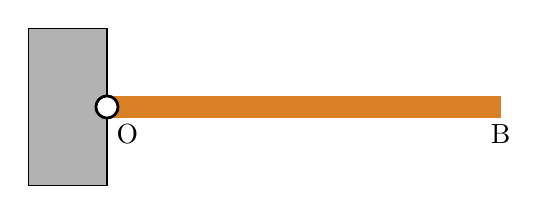
\begin{tikzpicture}
			\coordinate (O) at (0,0);
			\draw[fill=gray!60!white] (0,1) rectangle (-1,-1);
			\draw[line width=8pt, orange!40!brown] (0,0)--(5,0);
			\draw[line width=1pt, fill=white] (0,0) circle(4pt);
			\node[below right] at (0,-0.1) {O};
			\node[below] at (5,-0.1) {B};
		\end{tikzpicture}
	\end{center}
	\choice
	{$\SI{15}{\newton}$}
	{\True $\SI{25}{\newton}$}
	{$\SI{10}{\newton}$}
	{$\SI{30}{\newton}$}
	\loigiai{}
\end{ex}
% ===================================================================
\begin{ex}\mkstar{3}
	Một thanh đồng chất có chiều dài $L$, trọng lượng $\SI{200}{\newton}$, treo một vật có trọng lượng $\SI{450}{\newton}$ vào thanh như hình \ref{fig:23.5}. Các lực $\vec F_1$, $\vec F_2$ của thanh tác dụng lên hai điểm tựa có độ lớn lần lượt là
	\begin{center}
		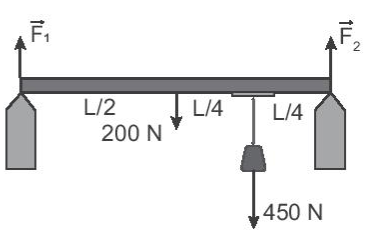
\includegraphics[width=0.4\linewidth]{../figs/VN10-2022-PH-TP023-P-5}
		\captionof{figure}{}
		\label{fig:23.5}
	\end{center}
	\choice
	{\True $\SI{212.5}{\newton}$; $\SI{437.5}{\newton}$}
	{$\SI{325}{\newton}$; $\SI{325}{\newton}$}
	{$\SI{437.5}{\newton}$; $\SI{212.5}{\newton}$}
	{$\SI{487.5}{\newton}$; $\SI{162.5}{\newton}$}
	\loigiai{Các lực thành phần theo phương $Oy$ cân bằng nhau:
		\begin{equation}
			\label{eq:23.1}
			F_1+F_2-200-450=0
		\end{equation}
		Áp dụng quy tắc moment lực đối với trục quay tại A:
		\begin{equation}
			\label{eq:23.2}
			\dfrac{L}{2}\cdot 200+\dfrac{3L}{4}\cdot 450=LF_2
		\end{equation}
		Từ (\ref{eq:23.1}) và (\ref{eq:23.2}), suy ra $F_1=\SI{212.5}{\newton}$, $F_2=\SI{437.5}{\newton}$.}
\end{ex}
% ===================================================================
\begin{ex}\mkstar{3}
Một đường ống đồng chất có trọng lượng $\SI{100}{\newton}$, chiều dài $L$, tựa trên điểm tựa như hình \ref{fig:23.3}. Khoảng cách $x$ và độ lớn phản lực $F_R$ của điểm tựa tác dụng lên đường ống là
\begin{center}
	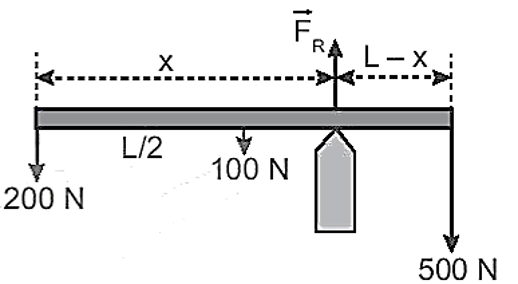
\includegraphics[width=0.4\linewidth]{../figs/VN10-2022-PH-TP023-P-3}
	\captionof{figure}{}
	\label{fig:23.3}
\end{center}	
	\choice
	{\True $x=0,69L$; $F_R=\SI{800}{\newton}$}
	{$x=0,69L$; $F_R=\SI{400}{\newton}$}
	{$x=0,6L$; $F_R=\SI{552}{\newton}$}
	{$x=0,6L$; $F_R=\SI{248}{\newton}$}
	\loigiai{Áp dụng quy tắc moment lực đối với trục quay tại A:
		\begin{center}
			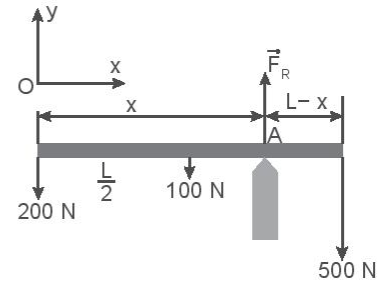
\includegraphics[width=0.4\linewidth]{../figs/VN10-2022-PH-TP023-P-4}
		\end{center}
		$$x\cdot 200+\left(x-\dfrac{L}{2}\right)\cdot100=\left(L-x\right)\cdot500$$
		$$\Rightarrow x=0,69L$$
		Các lực thành phần theo phương $Oy$:
		$$F_R-200-100-500=0\Rightarrow F_R=\SI{800}{\newton}.$$}
\end{ex}
% ===================================================================
\begin{ex}\mkstar{3}
	Một thanh chắn đường dài $\SI{7.8}{\meter}$, có trọng lượng $\SI{2100}{\newton}$ và có trọng tâm
	ở cách đầu bên trái $\SI{1.2}{\meter}$. Thanh có thể quay quanh một trục nằm ngang ở cách đầu bên trái $\SI{1.5}{\meter}$. Hỏi phải tác dụng vào đầu bên phải một lực có độ lớn tối thiểu bằng bao nhiêu để thanh ấy nằm ngang?
	\choice
	{\True $\SI{100}{\newton}$}
	{$\SI{200}{\newton}$}
	{$\SI{300}{\newton}$}
	{$\SI{400}{\newton}$}
	\loigiai{\begin{center}
			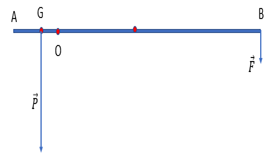
\includegraphics[width=0.4\linewidth]{../figs/VN10-2022-PH-TP023-P-1}
		\end{center}
		Áp dụng quy tắc moment cho trục quay qua O:
		$$P\cdot OG=F\cdot OB$$
		$$\Rightarrow F=\dfrac{P\cdot OG}{OB}=\dfrac{\left(\SI{2100}{\newton}\right)\cdot\left(\SI{0.3}{\meter}\right)}{\SI{7.8}{\meter}-\SI{1.5}{\meter}}=\SI{100}{\newton}.$$}
\end{ex}
% ===================================================================
\begin{ex}\mkstar{3}
Một tấm ván nặng $\SI{270}{\newton}$ được bắc qua một con mương. Trọng tâm của tấm ván cách điểm tựa trái $\SI{0.8}{\meter}$ và cách điểm tựa phải là $\SI{1.6}{\meter}$. Hỏi lực mà tấm ván tác dụng lên điểm tựa bên trái có độ lớn là bao nhiêu?	
	\choice
	{\True $\SI{180}{\newton}$}
	{$\SI{90}{\newton}$}
	{$\SI{160}{\newton}$}
	{$\SI{80}{\newton}$}
	\loigiai{\begin{center}
			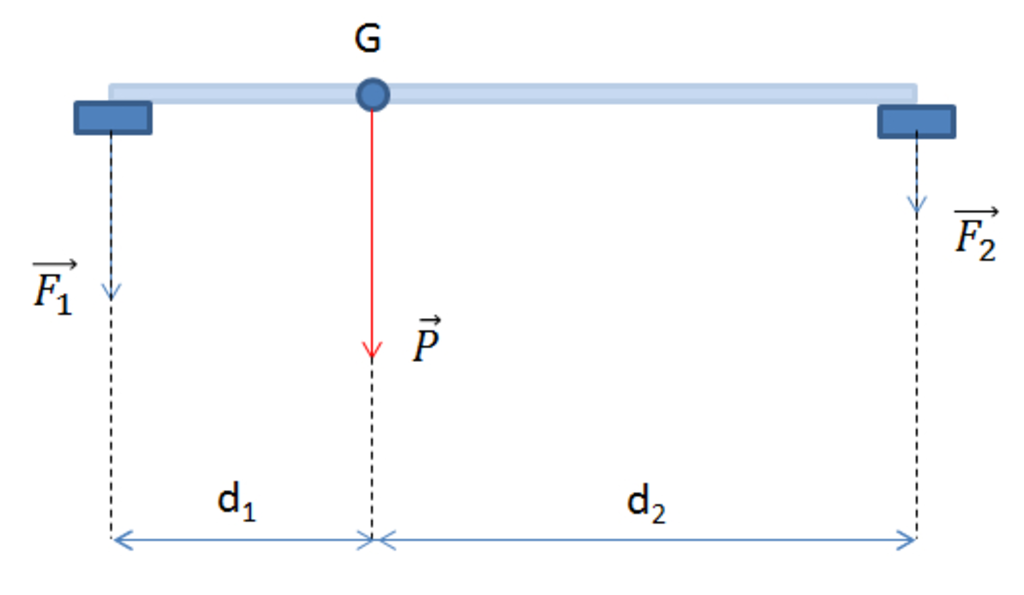
\includegraphics[width=0.4\linewidth]{../figs/VN10-2022-PH-TP023-P-2}
		\end{center}
		Áp dụng quy tắc moment cho trục quay qua điểm tựa phải:
		$$P\cdot d_2=F'_1\cdot\left(d_1+d_2\right)$$
		với $\vec F'_1=-\vec F_1$ là lực do điểm tựa trái tác dụng lên ván.
		$$\Rightarrow F'_1=\dfrac{P\cdot d_2}{d_1+d_2}=\SI{180}{\newton}$$
		Lực do ván tác dụng lên điểm tựa trái:
		$$F_1=F'_1=\SI{180}{\newton}.$$}
\end{ex}
% ===================================================================
\begin{ex}\mkstar{3}
	Một thanh nhẹ gắn vào sàn tại B như hình vẽ.
	\begin{center}
		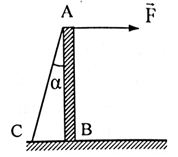
\includegraphics[scale=1]{../figs/VN10-2021-PH-TP021-6.png}
	\end{center}
	Tác dụng lên đầu A lực kéo $F=\SI{100}{N}$ theo phương ngang. Thanh được giữ cân bằng nhờ dây AC. Lực căng của dây có giá trị là bao nhiêu? Biết $\alpha = \SI{30}{\degree}$.
	\choice
	{$\SI{250}{N}$}
	{$\SI{150}{N}$}
	{$\SI{100}{N}$}
	{\True $\SI{200}{N}$}
	\loigiai{Chọn trục quay tại B. Áp dụng quy tắc moment lực:
		$$F \cdot \text{AB} = T \cdot \text{AB} \cdot \sin \alpha \Rightarrow T = \dfrac{F}{\sin \alpha} = \SI{200}{N}$$}
\end{ex}
% ===================================================================
\begin{ex}\mkstar{4}
	Bán cầu đồng chất khối lượng $\SI{100}{g}$. Trên mép bán cầu đặt một vật nhỏ khối lượng $\SI{7.5}{g}$. Hỏi mặt phẳng của bán cầu sẽ nghiêng góc $\alpha$ bao nhiêu khi nó cân bằng? Biết rằng trọng tâm bán cầu cách mặt phẳng của bán cầu một đoạn $3R/8$ (với $R$ là bán kính của bán cầu).
	\begin{center}
		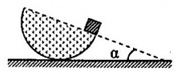
\includegraphics[scale=1]{../figs/VN10-2021-PH-TP021-7.png}
	\end{center}
	\choice
	{\True $11,31^\circ$}
	{$15^\circ$}
	{$20^\circ$}
	{$12^\circ$}
	\loigiai{	\begin{center}
			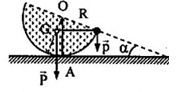
\includegraphics[scale=1]{../figs/VN10-2021-PH-TP021-8.png}
		\end{center}
		
		Các lực tác dụng lên bán cầu: trọng lực $\vec P$ của bán cầu, trọng lực $\vec p$ của vật nhỏ, phản lực $\vec Q$ tại điểm tiếp xúc A.
		
		Áp dụng quy tắc moment lực với trục quay qua O:
		$$P \cdot \text{OG} \cdot \sin \alpha = p \cdot R \cdot \cos \alpha \Rightarrow \tan \alpha = \dfrac{8m}{3M} \Rightarrow \alpha = 11,31^\circ$$}
\end{ex}
% ===================================================================
\begin{ex}\mkstar{4}
	Một cái thang có cấu tạo đồng đều được đặt dựa vào tường trơn nhẵn. 
	\begin{center}
		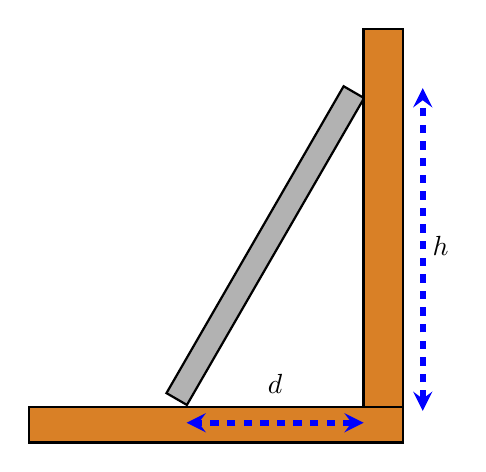
\begin{tikzpicture}
			\coordinate (O) at (0,0);
			\draw[stealth-stealth, line width=2pt, blue, dashed] (2,-2.1)--(2,2);
			
			\node [draw, thick, shape=rectangle, minimum width=0.3cm, minimum height=4.5cm, anchor=center, fill=gray!60!white, rotate=-30] at (O) {};
			\draw[line width=1pt, fill=orange!40!brown] (1.25,2.75) rectangle (1.75,-2.1);
			\draw[line width=1pt, fill=orange!40!brown] (1.75,-2.05) rectangle (-3,-2.5);
			\draw[stealth-stealth, line width=2pt, blue, dashed] (1.25,-2.25)--(-1,-2.25);
			\node[right] at (2,0) {$h$};
			\node[above] at (0.125,-2) {$d$};
		\end{tikzpicture}
	\end{center}
	Để thang không bị trượt thì hệ số ma sát tĩnh ở chỗ mặt tiếp xúc của thang với sàn nhà phải thỏa điều kiện
	\choice
	{$\mu\le\dfrac{d}{2h}$}
	{\True $\mu\ge\dfrac{d}{2h}$}
	{$\mu\le\dfrac{2h}{d}$}
	{$\mu\le\dfrac{2h}{d}$}
	\loigiai{
	\begin{center}
		\begin{tikzpicture}
			\coordinate (O) at (0,0);
			\draw[stealth-stealth, line width=2pt, blue, dashed] (2,-2.1)--(2,2);
			
			\node [draw, thick, shape=rectangle, minimum width=0.3cm, minimum height=4.5cm, anchor=center, fill=gray!60!white, rotate=-30] at (O) {};
			\draw[line width=1pt, fill=orange!40!brown] (1.25,2.75) rectangle (1.75,-2.1);
			\draw[line width=1pt, fill=orange!40!brown] (1.75,-2.05) rectangle (-3,-2.5);
			\draw[stealth-stealth, line width=2pt, blue, dashed] (1.25,-2.25)--(-1,-2.25);
			\node[right] at (2,0) {$h$};
			\node[below] at (0.125,-2.5) {$d$};
			\draw[red, line width=2pt, -stealth] (O)--($(O)-(0,1.5)$);
			\draw[red, line width=2pt, -stealth] (-1,-2)--(-1,0);
			\draw[red, line width=2pt, -stealth] (1.25,1.9)--(-0.5,1.9);
			\draw[red, line width=2pt, -stealth] (-1,-2)--(0,-2);
			\node[above,red] at (-0.25,-2) {$\vec{F}_{\text{msn}}$};
			\node[right,red] at (0,-1.25) {$\vec{P}$};
			\node[left,red]  at (-1,0) {$\vec{N}_1$};
			\node[left,red]  at (-0.5,1.9) {$\vec{N}_2$};
			\node[above right] at (1.25,1.9) {O};
		\end{tikzpicture}
	\end{center}
	Áp dụng quy tắc moment cho trục quay qua O:
	$$N_1d=F_{\text{msn}}h+P\cdot\dfrac{d}{2}$$
	Mà $N_1=P$ nên:
	$$F_{\text{msn}}h=P\cdot\dfrac{d}{2}\Rightarrow F_{\text{msn}}=P\cdot\dfrac{d}{2h}.$$
	Lại có:
	$$F_{\text{msn}}\le\mu N_1=\mu P\Rightarrow\mu \ge\dfrac{d}{2h}.$$
	}
\end{ex}
% ===================================================================
\begin{ex}\mkstar{4}
	Một thanh AB đồng chất, tiết diện đều có khối lượng $\SI{3}{\kilogram}$, dài $\SI{2}{\meter}$, có một đầu được gắn bởi một bản lề nhẵn vào trần nhà tại A. Đầu B được buộc vào một sợi dây nhẹ không đàn hồi. Đầu kia của sợi dây được gắn vào trần nhà ở điểm C. Thanh tạo một góc $\SI{30}{\degree}$ với phương ngang và sợi dây tạo một góc $\SI{60}{\degree}$ so với phương ngang như hình bên. 
	\begin{center}
		\begin{tikzpicture}
			\coordinate (A) at (0,0);
			\coordinate (B) at ($(A)+(-30:4)$);
			\coordinate (C) at (5,0);
			\tkzMarkAngle[size=0.75cm,color=blue,line width=1.5pt](B,A,C);
			\tkzLabelAngle[color=black,pos=1.2](B,A,C){$\SI{30}{\degree}$};
			\tkzMarkAngle[size=0.75cm,color=blue,line width=1.5pt](A,C,B);
			\tkzMarkAngle[size=0.65cm,color=blue,line width=1.5pt](A,C,B);
			\tkzLabelAngle[color=black,pos=1.2](A,C,B){$\SI{60}{\degree}$};
			\draw[line width=2pt] (A)--(B);
			\draw[line width=1pt, gray] (C)--(B);
			\draw[line width=6pt, gray] (-0.5,0)--(5.5,0);
			\node[above] at (A) {A};
			\node[above] at (C) {C};
			\node[below] at (B) {B};
		\end{tikzpicture}
	\end{center}
	Lấy $g=\SI{10}{\meter/\second^2}$. Lực căng của sợi dây có độ lớn là
	\choice
	{$\SI{7.5}{\newton}$}
	{$\SI{14}{\newton}$}
	{\True $\SI{13}{\newton}$}
	{$\SI{6.5}{\newton}$}
	\loigiai{}
\end{ex}
\Closesolutionfile{ans}
\section{Trắc nghiệm đúng/sai}
\setcounter{ex}{0}
\Opensolutionfile{ans}[ans/VN10-Y24-PH-SYL-023P-TF]
% ===================================================================
\begin{ex}\mkstar{1}
	Xét tính đúng/sai của các phát biểu sau đây khi nói về ngẫu lực.
	\choiceTF[t]
	{Ngẫu lực tác dụng vào một vật sẽ làm vật vừa quay vừa tịnh tiến}
	{Moment của ngẫu lực không chỉ phụ thuộc cánh tay đòn của ngẫu lực mà còn phụ thuộc khoảng cách từ lực đến trục quay}
	{Moment của ngẫu lực phụ thuộc điểm đặt mỗi lực hay vị trí trục quay}
	{\True Ngẫu lực không gây tác dụng lên trục quay}
	\loigiai{\begin{itemchoice}
			\itemch Sai. Ngẫu lực tác dụng vào một vật chỉ làm vật quay.
			\itemch Sai. Moment của ngẫu lực chỉ phụ thuộc cánh tay đòn của ngẫu lực.
			\itemch Sai. Moment của ngẫu lực không phụ thuộc điểm đặt mỗi lực hay vị trí trục quay.
			\itemch Đúng. Ngẫu lực không gây tác dụng lên trục quay.
	\end{itemchoice}}
\end{ex}
% ===================================================================
\begin{ex}\mkstar{2}
	Hai anh em Bình và An đang chơi trò bập bênh. Bập bênh là một tấm ván AB cứng, đồng chất, tiết diện đều và giá đỡ nằm ngay trọng tâm O của tấm ván. AB chia thành 6 đoạn bằng nhau (như hình). Khối lượng của An bằng $\SI{25}{\kilogram}$ còn khối lượng của Bình bằng $\SI{75}{\kilogram}$. An ngồi bên phần OA và Bình ngồi bên phần OB.
	\begin{center}
		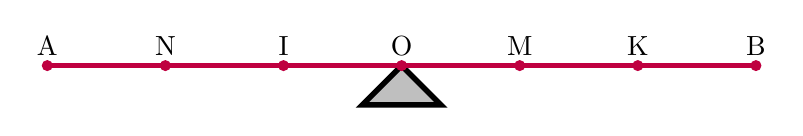
\begin{tikzpicture}
			\draw[line width=2pt, fill=gray!50!white] (0,0)--(-0.5,-0.5)--(0.5,-0.5)--(0,0);
			\draw[line width=2pt, purple] (-4.5,0)--(4.5,0);
			\foreach \i in {-4.5,-3,...,4.5}{
				\fill[fill=purple]   (\i,0) circle[radius=2pt];
			
			};
			\node[above] at (-4.5,0) {A};
			\node[above] at (-1.5,0) {I};
			\node[above] at (-3,0) {N};
			\node[above] at (0,0) {O};
			\node[above] at (1.5,0) {M};
			\node[above] at (3,0) {K};
			\node[above] at (4.5,0) {B};
		\end{tikzpicture}
	\end{center}
	\choiceTF[t]
	{\True Bập bênh trên không có moment trọng lực}
	{Khi Bình và An cùng ngồi tại hai đầu tấm ván thì moment trọng lực của hai anh em bằng nhau }
	{Khi Bình và An cùng ngồi tại hai đầu tấm ván thì bập bênh có xu hướng quay ngược chiều kim đồng hồ}
	{\True Khi An ngồi ở A, để bập bênh ở trạng thái cân bằng nằm ngang thì Bình phải dịch chuyển tới vị trí M}
	\loigiai{
	\begin{itemchoice}
		\itemch Đúng.
		\itemch Sai. Do $\mathrm{OA}=\mathrm{OB}$ và $m_{\text{Bình}}>m_{\text{An}}$ nên $M_{\vec{P}\text{An}}<M_{\vec{P}{\text{Bình}}}$.
		\itemch Sai. Do $M_{\vec{P}\text{An}}<M_{\vec{P}\text{Bình}}$ nên bập bênh có xu hướng quay cùng chiều kim đồng hồ.
		\itemch Đúng.
	\end{itemchoice}
	}
\end{ex}
% ===================================================================
\begin{ex}\mkstar{3}
	Một thanh ngang AB có khối lượng $\SI{4}{\kilogram}$ như hình bên. Đầu A của thanh treo một thùng hàng có khối lượng $\SI{50}{\kilogram}$. Thanh AB dài $\SI{3}{\meter}$ và có vạch chia đều. Lấy $g=\SI{10}{\meter/\second^2}$.
	\begin{center}
		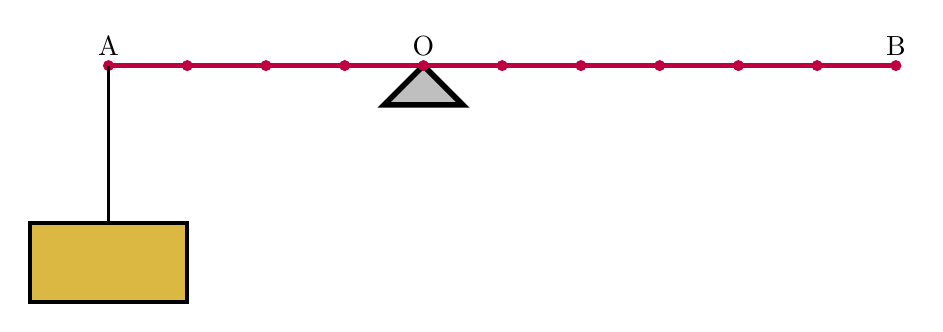
\begin{tikzpicture}
			\draw[line width=2pt, fill=gray!50!white] (0,0)--(-0.5,-0.5)--(0.5,-0.5)--(0,0);
			\draw[line width=2pt, purple] (-4,0)--(6,0);
			\foreach \i in {-4,-3,...,6}{
				\fill[fill=purple]   (\i,0) circle[radius=2pt];
				
			};
			\draw[line width=1pt] (-4,0)--(-4,-2);
			\draw[line width=1.5pt, fill=yellow!40!brown] (-5,-2) rectangle (-3,-3);
			\node[above] at(-4,0) {A};
			\node[above] at(0,0) {O};
			\node[above] at(6,0) {B};
		\end{tikzpicture}
	\end{center}
	\choiceTF[t]
	{Cánh tay đòn của moment trọng lực thùng hàng đối với trục quay O là $\SI{1.5}{\meter}$}
	{Thanh AB không có moment đối với trục quay tại O}
	{\True Moment của trọng lực thùng hàng đối với trục quay tại O bằng $\SI{600}{\newton\meter}$}
	{\True Để thanh cân bằng cần treo vào điểm chính giữa của OB một vật có khối lượng $m'=\xsi{\dfrac{196}{3}}{\kilogram}$}
	\loigiai{
	\begin{itemchoice}
		\itemch Sai. Cánh tay đòn của moment trọng lực thùng hàng đối với trục quay O là $\mathrm{OA}=\SI{1.2}{\meter}$.
		\itemch Sai. Thanh AB có $P=mg=\SI{40}{\newton}$ và điểm đặt của trọng lực tại I cách trục quay O đoạn $\mathrm{OI}=\SI{0.3}{\meter}$ nên có moment.
		\itemch Đúng.
		\itemch Đúng.
	\end{itemchoice}
	}
\end{ex}
\Closesolutionfile{ans}
\section{Tự luận}
\setcounter{ex}{0}
\Opensolutionfile{ans}[ans/VN10-Y24-PH-SYL-023P-TL]
\begin{ex}\mkstar{2}
	Biết các lực $F_1=\SI{25}{\newton}$, $F_2=\SI{10}{\newton}$, $F_3=\SI{10}{\newton}$ tác dụng vào thanh AB có trục quay tại A như hình vẽ.
	\begin{center}
		\begin{tikzpicture}
			\coordinate (B) at (0,0);
			\coordinate (A)  at ($(B)+(200:4)$);
			\coordinate (F1)  at ($(B)+(175:2.5)$);
			\coordinate (F3)  at ($(B)+(20:2)$);
			\coordinate (F2)  at ($(B)+(-70:2)$);
			\coordinate (C)  at ($(B)+(175:3.625)$);
			\tkzMarkRightAngle[size=0.3,color=red, line width=1pt](A,B,F2);
			\tkzMarkRightAngle[size=0.3, line width=1pt](A,C,B);
			\draw[line width=3pt] (A)--(B);
			\draw[dashed, line width=1pt] (A)--(C)--(B);
			\draw[blue, line width=2pt, -stealth] (B)--(F1);
			\draw[blue, line width=2pt, -stealth] (B)--(F2);
			\draw[blue, line width=2pt, -stealth] (B)--(F3);
			\fill   (A) circle[radius=4pt]  node [below left] {A};
			\node[above, blue] at (F1) {$\vec{F_1}$};
			\node[above, blue] at (F3) {$\vec{F_3}$};
			\node[right, blue] at (F2) {$\vec{F_2}$};
			\node[above] at (B) {B};
			\node[above] at (C) {C};
			\node[below] at ($(A)!0.5!(B)-(0,0.25)$) {$\SI{80}{\centi\meter}$};
				\tkzMarkAngle[size=0.75cm,color=red, line width=1pt](F1,B,A);
			\tkzLabelAngle[color=black,pos=1.2](F1,B,A){$\SI{25}{\degree}$};
			
		\end{tikzpicture}
	\end{center}
	\begin{enumerate}[label=\alph*)]
		\item Các lực $\vec{F}_1$; $\vec{F}_2$; $\vec{F}_3$ tác dụng lên thanh làm cho thanh quay theo chiều nào?
		\item Xác định cánh tay đòn của các lực $\vec{F}_1$; $\vec{F}_2$ và $\vec{F}_3$ đối với trục quay qua A.
		\item Tính độ lớn moment của các lực $\vec{F}_1$; $\vec{F}_2$; $\vec{F}_3$ đối với trục quay qua A.
	\end{enumerate}
	\loigiai{
	\begin{enumerate}[label=\alph*)]
		\item Lực $\vec{F}_1$ làm cho thanh quay ngược chiều kim đồng hồ.\\
		Lực $\vec{F}_2$ làm cho thanh quay cùng chiều kim đồng hồ.
		\\
		Lực $\vec{F}_3$ không có tác dụng làm cho thanh quay vì giá của lực đi qua trục quay.
		\item Cánh tay đòn của các lực:\\
		$d_1=\mathrm{AC}=\mathrm{AB}\sin\SI{25}{\degree}=\SI{0.338}{\meter}$\\
		$d_2=\mathrm{AB}=\SI{0.8}{\meter}$\\
		$d_3=0$.
		\item Moment của lực đối với trục quay qua A:\\
		$M_{F_1}=F_1d_1=\left(\SI{25}{\newton}\right)\cdot\left(\SI{0.8}{\meter}\right)\cdot\sin\SI{25}{\degree}=\SI{8.45}{\newton\meter}$.\\
		$M_{F_2}=F_2\cdot d_2=\left(\SI{10}{\newton}\right)\cdot\left(\SI{0.8}{\meter}\right)=\SI{8}{\newton\meter}$.
		\\
		$M_{F_3}=F_3d_3=0$.
	\end{enumerate}
	}
\end{ex}
% ======================================================================
\begin{ex}\mkstar{2}
	Một chiếc thước mảnh có trục quay nằm ngang đi qua trọng tâm O của thước. Dùng hai ngón tay tác dụng vào thước một ngẫu lực đặt vào hai điểm A và B cách nhau $\SI{4.5}{\centi\meter}$ và có độ lớn $F_{\mathrm{A}}=F_{\mathrm{B}}=\SI{1}{\newton}$.
	Thước quay đi một góc $\alpha=\SI{30}{\degree}$. Hai lực luôn luôn nằm ngang và vẫn đặt tại A và B (hình vẽ).
	\begin{center}
		\begin{tikzpicture}
			\coordinate (O) at (0,0);
			\coordinate (A) at ($(O)+(60:2)$);
			\coordinate (B) at ($(O)+(-120:2)$);
			\coordinate (FA) at ($(A)+(2,0)$);
			\coordinate (FB) at ($(B)+(-2,0)$);
			\coordinate (I) at ($(B)+(90:3.4641)$);
			\tkzMarkAngle[size=0.75cm,color=red, line width=1pt](A,B,I);
			\node [draw, thick, shape=rectangle, minimum width=0.3cm, minimum height=4.5cm, anchor=center, fill=gray!40!white, rotate=-30] at (O) {};
			\fill   (O) circle[radius=2pt]  node [right] {};
			\draw[line width=2pt, -stealth, line width=2pt, blue] (A)--(FA);
			\draw[line width=2pt, -stealth, line width=2pt, blue] (B)--(FB);
			\draw[dashed, line width=1pt] (B)--(I)--(A);
			\draw[dashed, line width=1pt] (0,-2)--(0,2);
			\node[right] at ($(B)+(0.2,0)$) {B};
			\node[above left] at ($(A)+(-0.2,0)$) {A};
			\node[right] at ($(O)+(0.2,0)$) {O};
			\node[above] at (I) {I};
			\node[above] at (FA) {$\vec{F}_{\mathrm{A}}$};
			\node[above] at (FB) {$\vec{F}_{\mathrm{B}}$};
			
			\tkzLabelAngle[color=black,pos=1.2](A,B,I){$\alpha$};
		\end{tikzpicture}
	\end{center}
	\loigiai{}
\end{ex}
% ======================================================================
\begin{ex}\mkstar{2}
	Thanh AB khối lượng $m$, chiều dài $L=\SI{3}{\meter}$ gắn vào tường với bản lề A. Đầu B của thanh treo vật nặng $\SI{5}{\kilogram}$. Thanh được giữ nằm ngang nhờ dây treo CD, biết lực căng dây $\SI{150}{\newton}$, $\mathrm{AC}=\SI{2}{\meter}$, dây treo hợp với thanh AB một góc $\alpha=\SI{45}{\degree}$ như hình vẽ bên dưới. 
	\begin{center}
		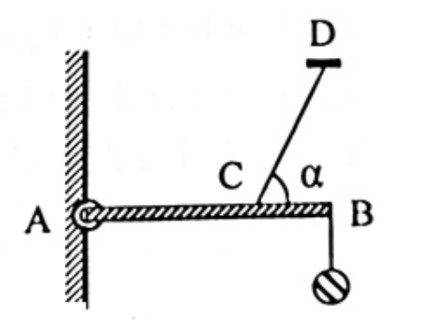
\includegraphics[width=0.25\linewidth]{../figs/VN10-2022-PH-TP023-P-11}
	\end{center}
	Xác định moment của lực căng dây CD và moment lực căng dây ở đầu B đối với trục quay qua A. Lấy $g=\SI{10}{\meter/\second^2}$.	
	\loigiai{
	Moment của lực căng dây:
	$M_{T_{\mathrm{B}/\mathrm{A}}}=T_{\mathrm{B}}\cdot\mathrm{AB}=m_{\mathrm{B}}g\cdot\mathrm{AB}=\SI{150}{\newton\meter}$.
	\\
	$M_{T_{\mathrm{CD}/\mathrm{A}}}=T_{\mathrm{CD}}\cdot\mathrm{AC}\sin\alpha=\xsi{150\sqrt{2}}{\newton\meter}$.
		}
\end{ex}
% ======================================================================
\begin{ex}\mkstar{2}
	Một cái thước $AB=\SI{1.2}{\meter}$ đặt trên mặt bàn nhẵn nằm ngang, có trục quay O cách đầu A một khoảng $\SI{80}{\centi\meter}$. Một lực $F_1=\SI{5}{\newton}$ tác dụng lên đầu A theo phương vuông góc với thước và lực thứ hai tác dụng lên đầu B của thước theo phương vuông góc với thước. Các lực đều nằm trên mặt phẳng nằm ngang. Nếu thước không chuyển động thì lực tác dụng vào đầu B của thước có hướng và độ lớn như thế nào?
		\begin{center}
		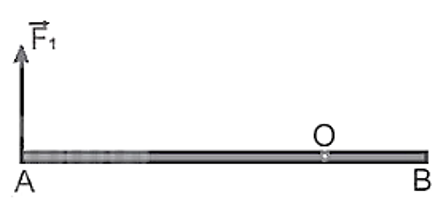
\includegraphics[width=0.35\linewidth]{../figs/VN10-2022-PH-TP023-P-8}
	\end{center}
	\loigiai{$\vec F_2$ cùng hướng với $\vec F_1$.\\
		Áp dụng quy tắc moment cho trục quay qua O:
		$$F_1\cdot OA=F_2\cdot OB\Rightarrow F_2=\dfrac{F_1\cdot OA}{OB}=\dfrac{\left(\SI{5}{\newton}\right)\cdot\left(\SI{0.8}{\meter}\right)}{\SI{0.4}{\meter}}=\SI{10}{\newton}.$$}
\end{ex}
% ======================================================================
\begin{ex}\mkstar{2}
	Một thanh kim loại đồng chất AB dài $\SI{2}{\meter}$ có tiết diện đều và khối lượng của thanh là $\SI{2}{\kilo\gram}$. Người ta treo vào đầu A của thanh một vật có khối lượng $\SI{5}{\kilogram}$, đầu B một vật có khối lượng $\SI{1}{\kilogram}$. Hỏi phải đặt một giá đỡ tại điểm O cách đầu A một khoảng là bao nhiêu để thanh cân bằng?
	\loigiai{\begin{center}
			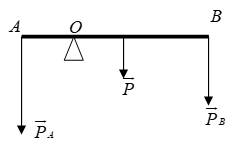
\includegraphics[width=0.3\linewidth]{../figs/VN10-2022-PH-TP023-P-9}
		\end{center}
		Gọi O là vị trí điểm tựa.\\
		Áp dụng quy tắc moment cho trục quay qua O:
		\begin{eqnarray*}
			&&P_\text{A}\cdot OA=P\cdot OG+P_\text{B}\cdot OB\\
			&\Leftrightarrow &P_\text{A}\cdot OA=P\cdot\left(\dfrac{AB}{2}-OA\right)+P_\text{B}\cdot\left(AB-OA\right)\\
			&\Leftrightarrow &50\cdot OA=20\cdot\left(1-OA\right)+10\cdot\left(2-OA\right)\\
			&\Rightarrow &OA=\SI{0.5}{\meter}.
	\end{eqnarray*}}
\end{ex}

% ======================================================================
\begin{ex}\mkstar{3}
	Một thanh sắt dài, đồng chất, tiết diện đều, được đặt trên bàn sao cho $\frac{1}{4}$ chiều dài của nó nhô ra khỏi bàn. Tại đầu nhô ra, người ta đặt một lực $\vec F$ thẳng đứng hướng xuống dưới. Khi lực đạt tới giá trị $\SI{40}{\newton}$ thì đầu kia của thanh sắt bắt đầu bênh lên. Hỏi trọng lượng của thanh sắt bằng bao nhiêu?
	\begin{center}
		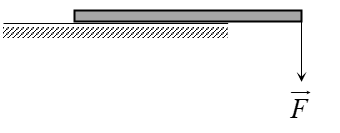
\includegraphics[width=0.4\linewidth]{../figs/VN10-2022-PH-TP023-P-10}
	\end{center}
	\loigiai{Áp dụng quy tắc moment với điểm tựa tại cạnh bàn:
		\begin{eqnarray*}
			&&P\cdot\left(\dfrac{L}{2}-\dfrac{L}{4}\right)=F\cdot\dfrac{L}{4}\\
			&\Rightarrow& F=P=\SI{40}{\newton}.
	\end{eqnarray*}}
\end{ex}
% ======================================================================
\begin{ex}\mkstar{3}
Một thanh có độ dài $L$, trọng lượng $\SI{10}{\newton}$, được treo nằm ngang vào tường như hình \ref{fig:23.6}. Một vật có trọng lượng $\SI{20}{\newton}$ treo ở đầu thanh. Dây treo hợp với thanh một góc $\alpha=\SI{30}{\degree}$. Xác định độ lớn lực căng dây treo.
\begin{center}
	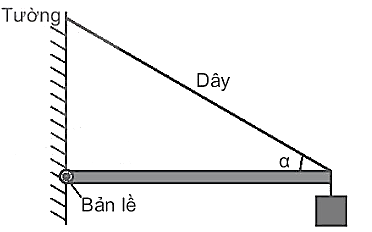
\includegraphics[width=0.4\linewidth]{../figs/VN10-2022-PH-TP023-P-6}
	\captionof{figure}{}
	\label{fig:23.6}
\end{center}	
	\loigiai{Áp dụng quy tắc moment đối với trục quay qua O:
		\begin{center}
			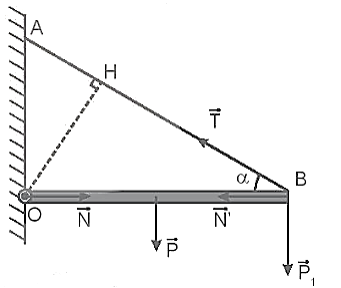
\includegraphics[width=0.35\linewidth]{../figs/VN10-2022-PH-TP023-P-7}
		\end{center}
		$$0\cdot N+OH\cdot T=\dfrac{L}{2}\cdot P+L\cdot P_1$$
		$$\Leftrightarrow T\cdot L\sin\alpha=\dfrac{L}{2}\cdot P+L\cdot P_1$$
		$$\Rightarrow T=\dfrac{\dfrac{P}{2}+P_1}{\sin\alpha}=\dfrac{\SI{5}{\newton}+\SI{20}{\newton}}{\sin\SI{30}{\degree}}=\SI{50}{\newton}.$$}
\end{ex}
% ======================================================================
\begin{ex}\mkstar{3}
	Dùng cân đòn để cân một vật. Vì cánh tay đòn của cân không thật bằng nhau nên khi đặt vật ở đĩa cân bên này thì người ta cân được $\SI{40}{\gram}$ nhưng khi đặt vật sang đĩa cân bên kia, người ta cân được $\SI{44.1}{\gram}$. Lấy $g=\SI{10}{\meter/\second^2}$.
	 Tìm khối lượng đúng của vật.
	\begin{center}
		\begin{tikzpicture}
			\coordinate (A) at (-4,0);
			\coordinate (B) at (3.8,0);
			\coordinate (O) at (0,0);
			\draw[line width=2pt, gray] (O)--($(O)+(-60:0.4)$)--($(O)+(-120:0.4)$)--(O);
			\draw[line width=2pt] (A) node [below]{A}--(O) node [above]{O}--(B) node[below] {B};
			\draw[line width=2pt] (A)--($(A)+(0,0.5)$);
			\draw[line width=2pt] (-4.5,0.5)--(-3.5,0.5);
			\draw[line width=1.5pt] (-4.5,0.5) ..controls (-4.85,0.75)..(-4.75,1);
			\draw[line width=1.5pt] (-3.5,0.5) ..controls (-3.15,0.75)..(-3.25,1);
			\draw[line width=2pt] (3.3,0.5)--(4.3,0.5);
			\draw[line width=1.5pt] (3.3,0.5) ..controls (2.95,0.75)..(3.05,1);
			\draw[line width=1.5pt] (4.3,0.5) ..controls (4.65,0.75)..(4.55,1);
			\draw[line width=2pt] (B)--($(B)+(0,0.5)$);
			\filldraw[orange!40!brown] (-4,1) circle (0.475);
			\filldraw[orange!40!brown] (3.8,1) circle (0.475);
		\end{tikzpicture}
	\end{center}
	\loigiai{
	Gọi $m$ là khối lượng vật.\\
	Áp dụng quy tắc moment cho trục quay qua O:
	$$\begin{cases}
		P\cdot\mathrm{OA}=P_1\cdot\mathrm{OB}\\
		P_2\cdot\mathrm{OA}=P\cdot\mathrm{OB}
	\end{cases}\Rightarrow \dfrac{P}{P_2}=\dfrac{P_1}{P}.$$
	Như vậy:
	$$m=\sqrt{m_1m_2}=\SI{42}{\gram}.$$
	}
\end{ex}
% ======================================================================
\begin{ex}\mkstar{4}
	Một vật rắn phẳng, mỏng, có dạng là một hình vuông ABCD, mỗi cạnh là $a=\SI{10}{cm}$. Người ta tác dụng một ngẫu lực nằm trong mặt phẳng của hình vuông. Biết các lực vuông góc với đường chéo AD có độ lớn $\SI{10}{N}$ và đặt vào hai đỉnh của A và D. Tính moment của ngẫu lực.
	\loigiai{Ta có đường chéo của hình vuông:
		$$d=\sqrt{a^2 + a^2} = \SI{14.14}{cm} = \SI{0.14}{m}$$
		
		Moment ngẫu lực:
		$$M=Fd = \SI{1.41}{Nm}$$}
\end{ex}
\Closesolutionfile{ans}
